\subsection{Structure from motion}
Kolejnym etapem projektu było wykorzystanie techniki \textit{Structure from Motion} (SfM) do wyznaczania
struktur przestrzennych scen na podstawie dobranych zestawów zdjęć dwuwymiarowych. 

Algorytmy SfM, identyfikując i łącząc 
punkty wspólne między zdjęciami, ustalają zarówno rozmieszczenie tych punktów w przestrzeni, jak i pozycje 
i orientacje kamer, z których wykonano zdjęcia. Proces ten pozwala na oszacowanie struktury trójwymiarowej
sfotografowanego obszaru, czyli wygenerowanie chmury punktów odwzorowującej scenę w postaci 
zbioru punktów 3D o przypisanych kolorach, tak jak to pokazuje ilustracja \ref{fig:sfm_ex}. 

Do realizacji tego zadania użyto popularnego narzędzia COLMAP, a konkretnie jego wersji w formie biblioteki 
\textit{pycolmap}, oferującej funkcjonalności m.in. do wykrywania charakterystycznych cech na obrazach, 
łączenia punktów wspólnych na zdjęciach czy przeprowadzania rekonstrukcji sceny 3D na podstawie dopasowań 
między nimi.

Uzyskana chmura punktów jest dodatkowo poddawana filtracji z wykorzystaniem metod opartych na analizie 
sąsiedztwa każdego punktu. Proces ten pozwala na eliminację szumów poprzez usunięcie punktów, które nie 
wpisują się w lokalne wzorce przestrzenne. Tak przygotowana trójwymiarowa reprezentacja sceny służy za 
podstawę do modelowania z zastosowaniem algorytmu Gaussian Splatting.

\begin{figure}[!ht]
    \centering
    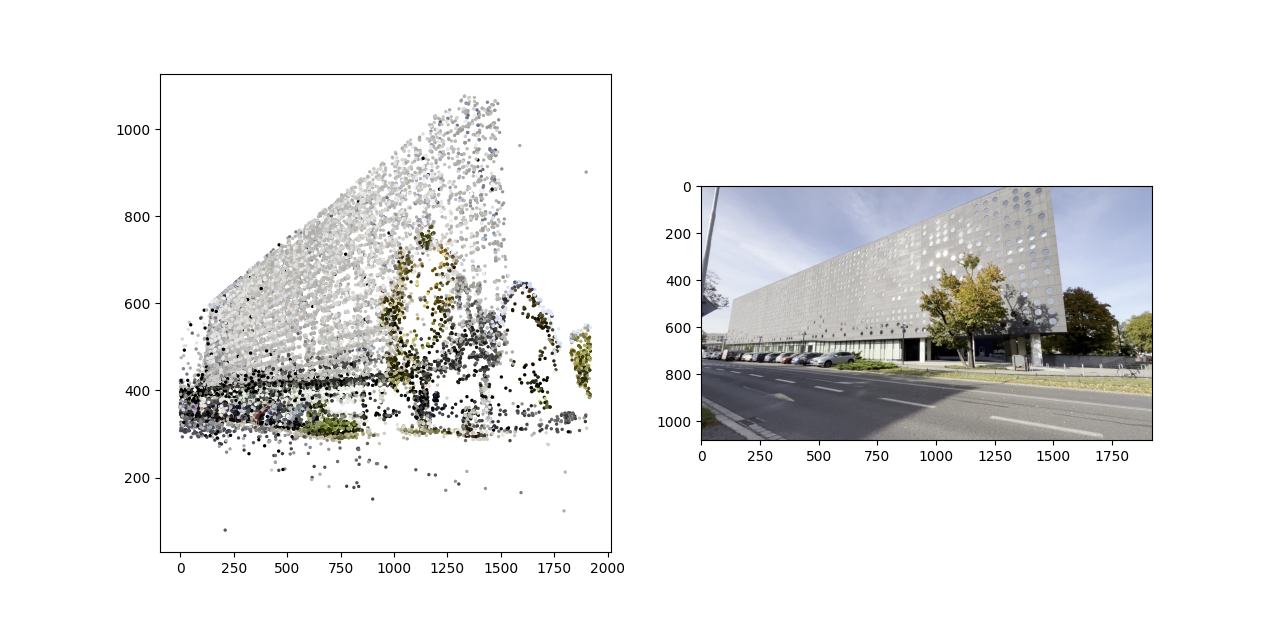
\includegraphics[width=0.9\linewidth]{images/sfm.png}
    \caption{Projekcja przykładowej chmury punktów na płaszczyznę porównana do zdjęcia}
    \label{fig:sfm_ex}
\end{figure}